\begin{figure}[tbh]
	\centering
	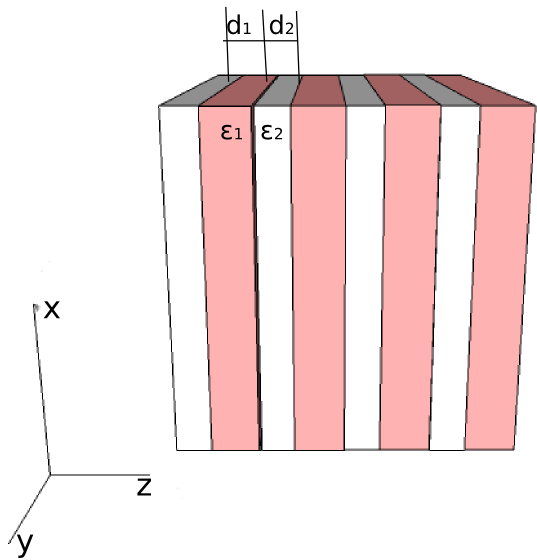
\includegraphics[width=.5\textwidth]{images/multilayer/multilayer-3d.png}
	\caption{Schemat wielowarstwy metaliczno dielektrycznej}
	\label{fig:mulschem}
\end{figure}


Zgodnie z~przedstawionymi własnościami materiałowymi, obrazowanie z~rozdzielczością przekraczającą klasyczne ograniczenie dyfrakcyjne za pomocą metali wiąże się z~dużymi stratami natężenia światła w~wyniku absorpcji\footnote{Dzieje się tak, ponieważ interesujące nas własności E-M materiałów obserwujemy dla długości fali w~okolicach rezonansów, w~których z~kolei materiały charakteryzują się wysoką absorpcją promieniowania}. Zwiększenie współczynnika transmisji przez wielowarstwy zawierające metal możliwe jest dzięki wykorzystaniu efektu rezonansowego tunelowania \cite{scalora-transparentmetal}. Chociaż zastosowanie zaproponowane w~cytowanej pracy nie było związane z~obrazowaniem, to możliwość uzyskania współczynnika transmisji rzędu 70\% dla wielowarstwy zawierającej łącznie 40~nm srebra świadczy także o~możliwości uzyskania obrazowania nadrozdzielczego przy zachowaniu wysokiej transmisji. 

Proponowaną konstrukcję wielowarstwy przedstawia schemat na rysunku \ref{fig:mulschem}. W omawianym podejściu obrazowanie nad rozdzielcze nie wynika wprost z~zastosowania materiału o~$\varepsilon = -1$, ale z~efektywnych anizotropowych właściwości powstałego w~ten sposób  metamateriału \cite{ramakrishna2003imaging}. Za pomocą przybliżenia ośrodka efektywnego, szerzej omówionego w~rozdziale \ref{subart:effmedium}, możemy dobierając grubości warstw do parametrów stosowanych materiałów we wzorach (\ref{eq:effmedium}) i~(\ref{eq:effmedium-mu})  uzyskać metamateriał o~$\varepsilon_z \to \infty$ i~$\varepsilon_x \to 0$.



\begin{figure}[tbh]
	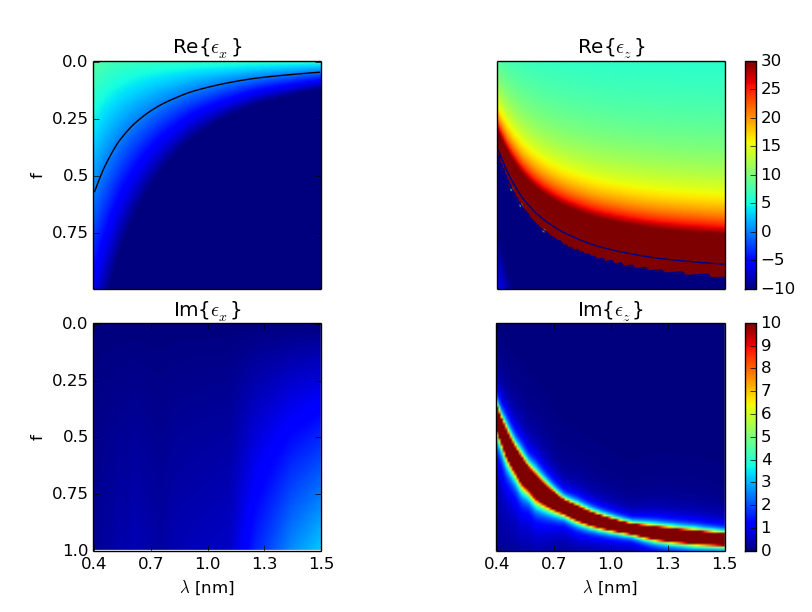
\includegraphics[width=\textwidth]{images/multilayer/agtio2-effective.png}
	\caption{Przenikalność ośrodka efektywnego obliczona zgodnie ze wzorem (\ref{eq:effmedium})  zbudowanego z~warstw $Ag$ \cite{PhysRevB.6.4370} i~$TiO_2$ \cite{DEVORE:51}. Współczynnik wypełnienia f=1 oznacza, że struktura zbudowana jest jedynie ze srebra. Konturem zaznaczono $\varepsilon_x=0$ oraz $\varepsilon_z=100$.}
	\label{fig:multiex}
%generacja rysuknu:
%./effEpsilon.py database/main/Ag/Johnson.yml database/main/TiO2/Devore-o.yml
\end{figure}

Przykładem materiałów, z~których w~opisany sposób można konstruować wielowarstwę charakteryzującą się transmisją bezdyfrakcyjną są $Ag$ i~$TiO_2$. Efektywne właściwości $\varepsilon$ i~$\mu$ dla wielowarstwy z~nich zbudowanej prezentują wykresy na rysunku \ref{fig:multiex}.~W szczególności na wykresach zaobserwować możemy, że obszar wysokiego $\varepsilon_z$ graniczy z~obszarem, w~którym ta składowa przenikalności elektrycznej przyjmuje wartości ujemne. Dla uzyskania własności bezdyfrakcyjnych, kluczowe jest dobranie takiego współczynnika wypełnienia~$f$, który pozwoli dla wybranych długości fali uzyskać efektywne wartości składowych tensora przenikalności elektrycznej jak najbliższe oczekiwanym.~W przypadku prezentowanych materiałów dla długości fali ok.~$500$~nm możemy uzyskać $\varepsilon_x \approx 0$ i~$\varepsilon_z \approx 10$.







